\chapter{Analiza wydajnościowa}

\section{Metody mierzenia wydajności aplikacji internetowych}
Głównym problemem aplikacji internetowych jest sytuacja, gdy w jednym momencie próbuje z niej skorzystać duża ilość użytkowników. Błędy aplikacji objawiają się wtedy poprzez długi czas przetwarzania, błąd przetwarzania bądź też odrzucenie zapytania HTTP. Oczywiście takie zachowanie jest bardzo niepożądane, dlatego też nowoczesne frameworki starają się minimalizować możliwość wystąpienia takich sytuacji.

Z tego też powodu aplikacjie poddawane są testom obciążeniowym. Tego typu testy opierają się na symulacji dużej liczby użytkowników próbujących skorzystać z aplikacji i analizie odpowiedzi z aplikacji. Na podstawie testów można uzyskać dane m.in. na temat:
\begin{itemize}
  \item procentowej ilości błędów,
  \item wartości minimalnej, maksymalnej, średniej i medianie czasu odpowiedzi,
  \item rozmiaru odpowiedzi z serwera,
  \item średniej ilości przetworzonych zapytań w jednostce czasu.
\end{itemize}


\section{Wyniki badań}
Badania zostały przeprowadzone na serwerze \emph{VPS} firmy \emph{DigitalOcean}. Posiada ona następujące parametry:
\begin{itemize}
  \item procesor: dwurdzeniowy Intel(R) Xeon(R) CPU E5-2650L v3 @ 1.80GHz,
  \item pamięć RAM: 2GB,
  \item dysk: 40GB SSD,
  \item system operacyjny: Ubuntu 16.04.2 LTS (Xenial Xerus)
\end{itemize}

Zgodnie z zaprojektowanym środowiskiem eksperymentalnym, testy wydajnościowe zostały przeprowadzone z wykorzystaniem narzędzia \emph{Locust}. Wyniki badań są uśrednionymi wartościami z 10 przebiegów testowych.

\subsection{Czas odpowiedzi z serwera}
W kategorii czasu odpowiedzi z serwera mierzone były następujące wartości:
\begin{itemize}
  \item mediana czasu odpowiedzi,
  \item średnia czas odpowiedzi,
  \item minimalny czas odpowiedzi,
  \item maksymalny czas odpowiedzi.
\end{itemize}

Wyniki dla poszczególnych frameworków przedstawione są w tabeli \ref{tab:czas_odp}.

\begin{table}[h]
\centering
\caption{Wyniki badań czasu odpowiedzi.\\Źródło: opracowanie własne.}
\label{tab:czas_odp}
\begin{tabular}{|l|l|l|l|l|}
\hline
              & \textbf{Mediana {[}ms{]}} & \textbf{Średnia {[}ms{]}} & \textbf{Min {[}ms{]}} & \textbf{Max {[}ms{]}} \\ \hline
\textbf{Ruby on Rails} & 160000           & 184060           & 114          & 544870       \\ \hline
\textbf{Phoenix}       & 23000            & 31873            & 623          & 169825       \\ \hline
\textbf{Express}       & 32000            & 33193            & 1514         & 112874       \\ \hline
\end{tabular}
\end{table}

Już podczas analizy wyników w formie tabelarycznej można zauważyć dużo większe wartości przy frameworku \emph{Ruby on Rails}. Różnice te są dużo bardziej widoczne na zestawieniu pokazanym w formie wykresu słupkowego przedstawionego na rysunku \ref{fig:response_times}.
\newpage
\begin{figure}[h]
  \centering
  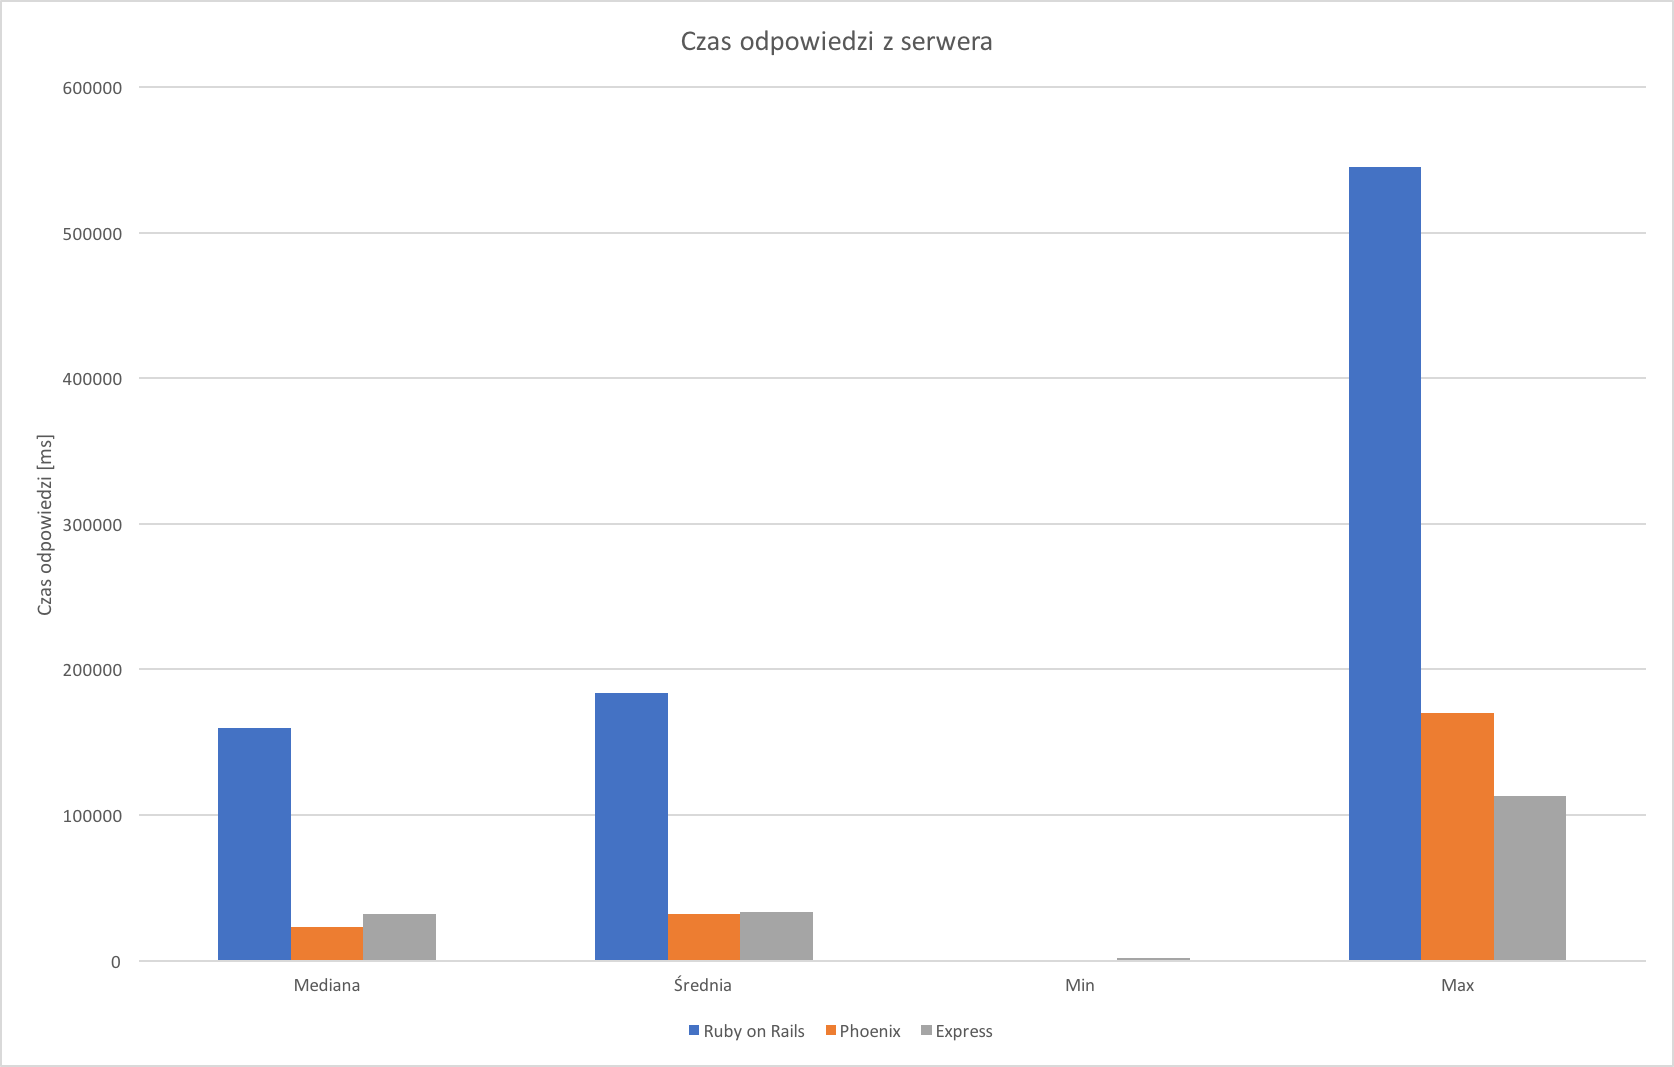
\includegraphics[width=\linewidth]{images/response_times}
  \caption{Porównanie czasów odpowiedzi z serwera.\\Źródło: opracowanie własne.}
  \label{fig:response_times}
\end{figure}

Zgodnie z przewidywaniami, \emph{Ruby on Rails} jest najwolniejszym frameworkiem, jeśli chodzi o czas odpowiedzi z serwera. Średni czas odpowiedzi jest ok. 5,5 razy większy niż w przypadku pozostałych frameworków. Spowodowane jest to faktem, iż język \emph{Ruby} nie należy do najszybszych języków programowania. Jego celem miało być dostarczenie przyjemności z programowania, co niestety odbiło się negatywnie na wydajności.

Najszybszym frameworkiem okazał się, zgodnie z oczekiwaniami, \emph{Phoenix}. Twórcom udało się zrealizować założenie dotyczące wydajności tego frameworka. Wpływ ma na to oczywiście wspomniany wcześniej język \emph{Elixir}. Co ciekawe, wydajność ta została osiągnięta z zachowaniem przyjemności z tworzenia aplikacji, co potwierdza duży potencjał tego frameworka.

Zaskoczeniem jest wydajność frameworka \emph{Express}. W zestawieniu jest on minimalnie wolniejszy od \emph{Phoenix'a}, co można określić jako bardzo dobry wynik. Wpływ na to ma minimalizm tego narzędzia. \emph{Express} z racji na swoją ,,ubogość'' domyślnych bibliotek jest bardzo małym frameworkiem. W połączeniu z szybką platformą \emph{Node.js}, która odpowiedzialna jest za serwowanie aplikacji, otrzymane zostały bardzo dobre wyniki czasu odpowiedzi.

\subsection{Ilość obsłużonych zapytań na sekundę}
Poza czasem odpowiedzi bardzo ważnym parametrem jest ilość obsłużonych zapytań na sekundę. Analiza tego parametru pozwala określić ilu użytkowników może jednocześnie korzystać z systemu bez problemów z wydajnością. Efektem owej analizy może być decyzja o zwiększeniu mocy obliczeniowej maszyny, która obsługuje aplikację bądź też zastosowanie \emph{load balancing'u}. Wyniki przeprowadzonych badań zostały przedstawione w tabeli \ref{tab:rps} oraz na wykresie \ref{fig:rps}.

\begin{table}[h]
\centering
\caption{Wyniki badań ilości zapytań na sekundę.}
\label{tab:rps}
\begin{tabular}{|l|l|}
\hline
                       & \textbf{RPS} \\ \hline
\textbf{Ruby on Rails} & 4,74         \\ \hline
\textbf{Phoenix}       & 9,86         \\ \hline
\textbf{Express}       & 22,09        \\ \hline
\end{tabular}
\end{table}

\begin{figure}[h]
  \centering
  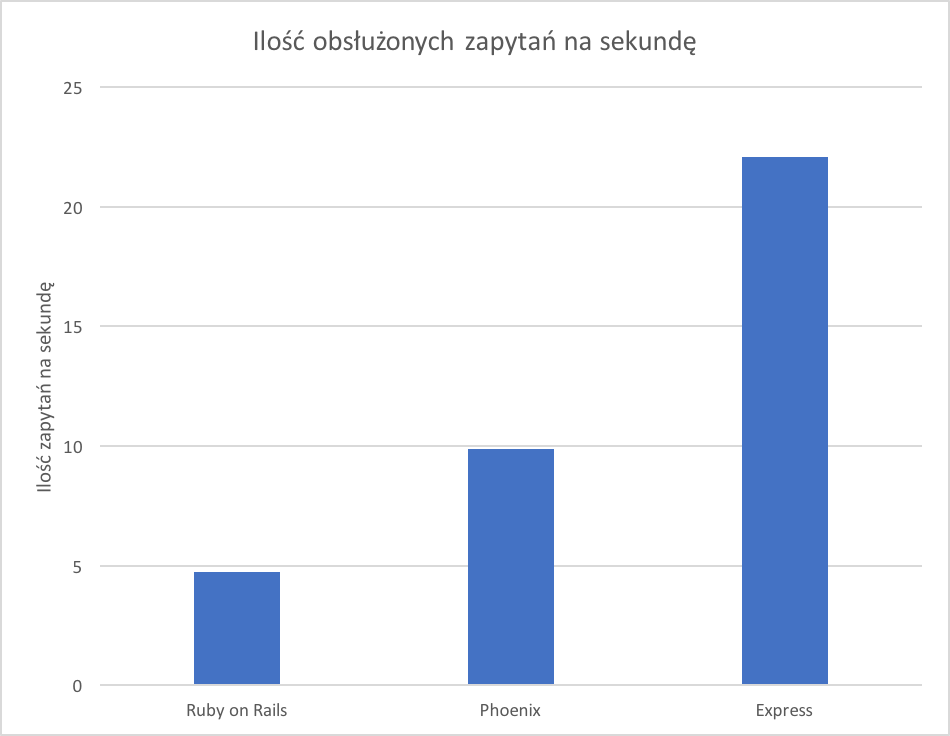
\includegraphics[width=0.7\linewidth]{images/rps}
  \caption{Porównanie ilości obsłużonych zapytań na sekundę.\\Źródło: opracowanie własne.}
  \label{fig:rps}
\end{figure}

Wyniki tych badań są nieco zaskakujące. Najwięcej zapytań, z ponad dwukrotnie lepszym wynikiem niż drugi w zestawieniu \emph{Phoenix}, obsłużył framework \emph{Express}. Przyczyn takiego wyniku ponownie można doszukiwać się w platformie \emph{Node.js}, na której oparty jest ten framework. Jest ona bardzo stabilna i stanowi podstawę dla wielu frameworków, w tym frontendowych, co doprowadziło do optymalizacji wydajności.

Drugi pod względem ilości przetworzonych zapytań na sekundę jest framework \emph{Phoenix}. Przed przeprowadzeniem testów, framework ten był faworytem w osiągnięciu najlepszego wyniku ze względu na język \emph{Elixir}, który pochodzi od \emph{Erlang'a}, a więc jest językiem posiadającym mechanizm \emph{lekkich wątków} (mechanizm podobny do \emph{zielonych wątków}). Testy jednak jednoznacznie pokazały, iż ilość obsłużonych zapytań w czasie sekundy nie jest wyjątkowo duża.

Frameworkiem, który zdołał obsłużyć najmniej zapytań w ciągu sekundy, został \emph{Ruby on Rails}. Także w tym przypadku taki wynik był zgodny z przewidywaniami. \emph{Ruby on Rails} jest 2 razy wolniejszy od \emph{Phoenix'a} i aż 4 razy wolniejszy od \emph{Express'a}. Pokazuje to, że framework ten, zgodnie z jego założeniami, powinien być stosowany głównie w celu prototypowania aplikacji.

\subsection{Poprawność odpowiedzi z serwera}
Poza szybkością działania aplikacji, bardzo ważnym elementem aplikacji internetowych jest ich niezawodność. Nawet jeśli framework jest wydajny, to traci on na wartości, jeśli nie jest niezawodny. W tym celu przeprowadzone zostały badania niezawodności. Ich wynikiem jest procentowa ilość błędów w odniesieniu do ilości zapytań. Wyniki w formie tabelarycznej oraz wykresu są przedstawione poniżej.

\begin{table}[h]
\centering
\caption{Wyniki ilości błędów zapytań w odniesieniu do ilości zapytań.}
\label{tab:poprawnosc}
\begin{tabular}{|l|l|}
\hline
                       & \textbf{Ilość błędów [\%]} \\ \hline
\textbf{Ruby on Rails} & 0,41         \\ \hline
\textbf{Phoenix}       & 9,01         \\ \hline
\textbf{Express}       & 0,00        \\ \hline
\end{tabular}
\end{table}

\newpage

\begin{figure}[h]
  \centering
  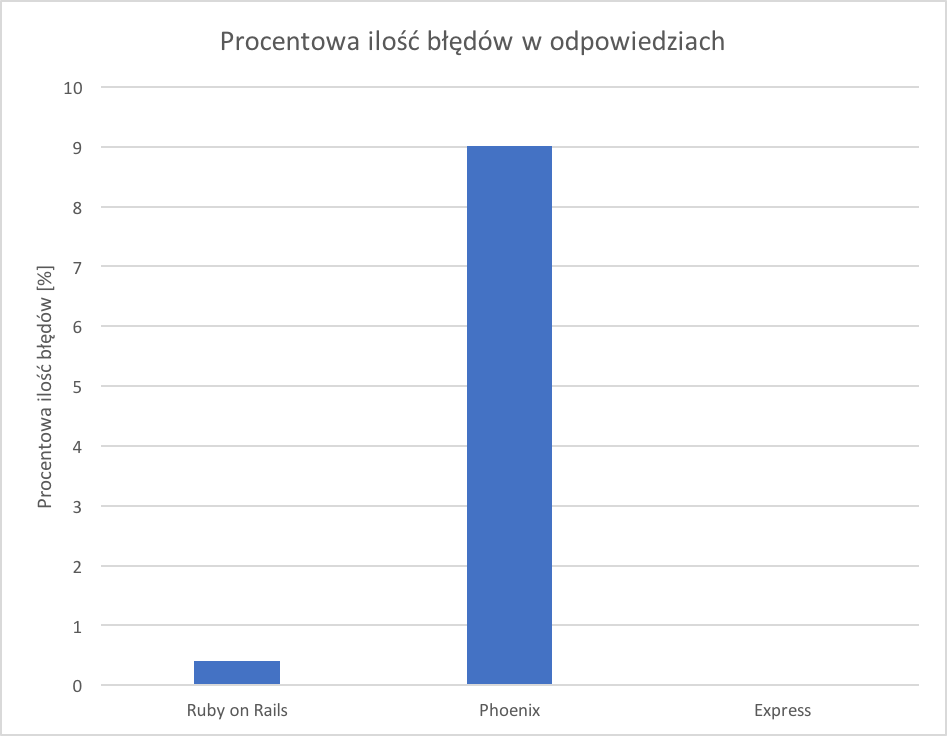
\includegraphics[width=0.7\linewidth]{images/errors}
  \caption{Zestawienie ilości błędnych odpowiedzi z serwerów.\\Źródło: opracowanie własne.}
  \label{fig:rps}
\end{figure}

Wyniki otrzymane na podstawie badań odpowiadają przewidywanym wynikom. \emph{Ruby on Rails} osiągnąl ilość błędów na poziomie $0,41\%$. Jest to wynik bardzo dobry, biorąc pod uwagę obciążenie, któremu została poddana aplikacja. I stanowczo jest to wynik mieszczący się w dopuszczalnych granicach błędów, które nie wpływają negatywnie na odczucia użytkownika.

Niewielką niespodzianką jest wynik frameworka \emph{Phoenix}. $9\%$ błednych odpowiedzi jest dużą wartością. Wynik ten można tłumaczyć jedynie młodym wiekiem tego rozwiązania, ponieważ \emph{Elixir} z założenia stawia na niezawodność. Stanowczo jest to element, który powinien zostać dopracowany w kolejnych wersjach frameworka.

Wręcz idealny wynik osiągnął \emph{Express}. W trakcie badań jego ilość błędów utrzymywała się na poziomie $0\%$, co oznacza pełną niezawodność. Przyczyną takiego wyniku jest niewątpliwie niewielki rozmiar frameworka. Oczywistym jest, że im mniej elementów może wygenerować błąd, tym większa niezawodność systemu.

\section{Wnioski z badań}
Na podstawie badań można wysnuć kilka wniosków. Po pierwsze - założenia frameworka nie zawsze pokrywają się z rzeczywistością. Przykładowo, \emph{Phoenix} reklamowany jest jako framework stawiający na szybkość działania, skalowalność i niezawodność. W przypadku pierwszych dwóch własności cel został osiągnięty (chociaż np. w porównaniu do \emph{Express'a} nie jest to wynik dużo lepszy). Problemem jest niestety niezawodność. Nawet najszybszy framework nie będzie wykorzystywany w momencie, kiedy nie jest niezawodny.

Po drugie, minimalizm, szczególnie pod względem wydajności, jest korzystny. Oczywiście taką aplikację trudniej się pisze oraz jest ryzyko, że mimo wszystko rozrośnie się do dużych rozmiarów. Mimo wszystko jeśli ktoś poszukuje wydajności, powinien skorzystać z \emph{Express'a} lub podobnych do niego frameworków.
